\documentclass[UTF8]{ctexart}
\usepackage{graphicx}
\usepackage{float}
%\usepackage{geometry}
%\geometry{
%	a4paper,
%	total={170mm,257mm},
%	left=20mm,
%	top=20mm
%}
%opening
\title{系统分析与设计方法 \\ 作业 1}
\author{软件42 \\ 欧阳鹏程 \\ 2141601030}

\begin{document}

\maketitle

\begin{enumerate}
	\item{一般地,面向对象分析与设计中存在三种事件处理的机制,除了普通的方法调用外,常常用到回调函数,而J2EE中还提供了一种基于监听方式的事件处理机制,请查阅资料,对Action以及ActionListener的机制进行分析,完成一个分析示例。}
	
	\paragraph{答:}
	Java中的事件监听是整个Java消息传递的基础和关键。牵涉到三类对象:事件源(Event Source)、事件(Event)、事件监听器(Event Listener)。 
	
	事件源是事件发生的场所,通常就是各个组件,它可以是一个按钮,编辑框等。 
	
	事件监听者负责监听事件源所发生的事件,并对各种事件做出相应的响应。 
	
	事件是描述事件源状态改变的对象。 
	
	\begin{figure}[H]
		\centering
		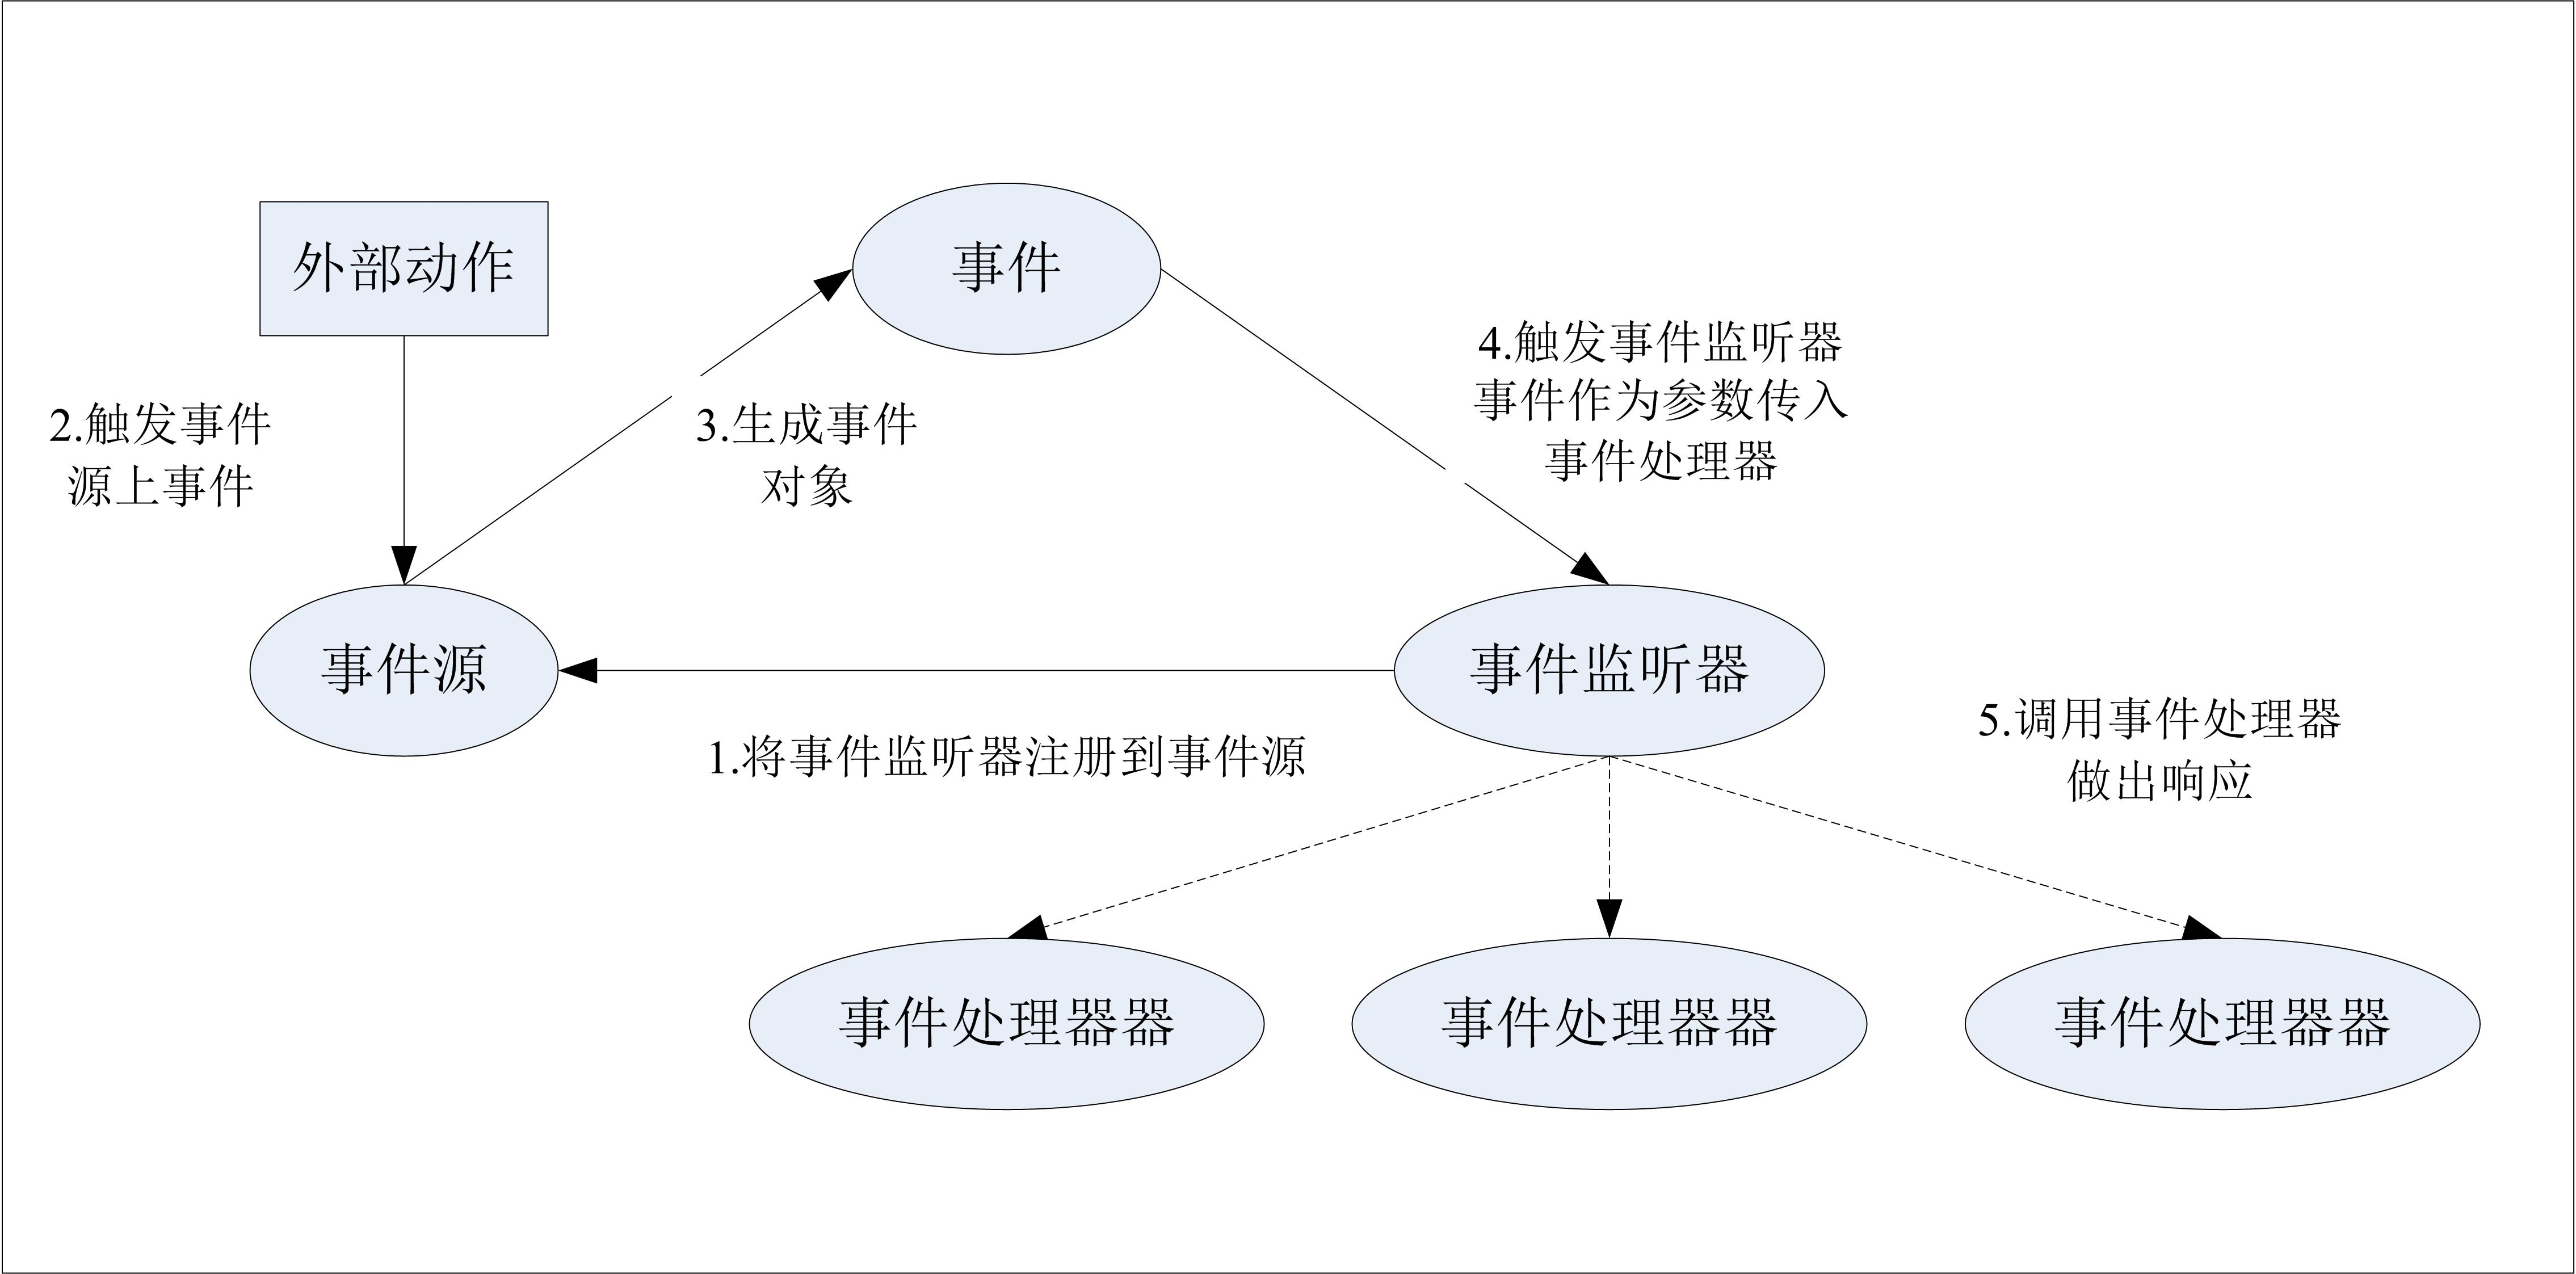
\includegraphics[width=\textwidth]{1.jpg}
		\caption{相互之间关系}
	\end{figure}

	其实现机制是先将一个监听器和一个监听对象绑定,当事件发生时,监听对象通知所有绑定了它的监听器,监听器收到消息后执行相应逻辑。正如以下时序图所示:
	
	\begin{figure}[H]
		\centering
		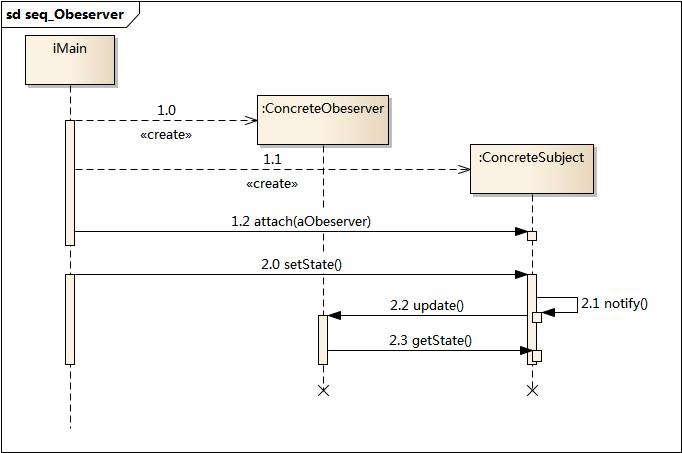
\includegraphics[width=\textwidth]{2.jpg}
		\caption{时序图}
	\end{figure}
\end{enumerate}


\end{document}
